\section{\'Evolution de la population de deux communes}
	
	
	Le graphique ci-dessous représente l'évolution du nombre d'habitants de deux communes voisines, nommées A et B, de l'année 1986 à l'année 2010 (de quatre années en quatre années) .
	
	\begin{center}
		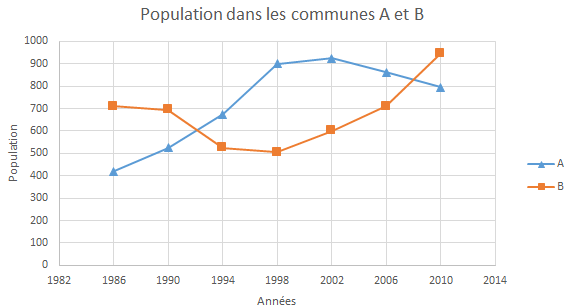
\includegraphics[scale=0.7]{./graph}
	\end{center}


\subsection{Lecture graphique}				

Répondre aux questions suivantes en utilisant uniquement le graphique ci-dessus.

\begin{questions}
	\question En quelle année, la population de la commune A a été maximale ?
	\begin{solution}
		La population de la commune A a été maximale en 2002.
	\end{solution}
	
	\question Préciser les années où les deux communes on eu le même nombre d'habitants.
	\begin{solution}
		Les deux villes ont eu la même population en 1992 et 2008.
	\end{solution}
	
	\question Quelles sont les périodes où la commune B a eu plus d'habitants que la commune A.
	\begin{solution}
		La commune B a eu plus d'habitants que la commune A entre 1986 et 1992 et entre 2008 et 2010.
	\end{solution}
	
	\question En quelle année l'écart entre le nombre d'habitants des deux communes a-t-il été le plus important.
	\begin{solution}
		L'écart entre les deux communes a été le plus important en 1998.
	\end{solution}
	
	\question Préciser, en justifiant la réponse, pendant quelle période de quatre années, la commune A a eu la plus forte augmentation de sa population.
	\begin{solution}
		La plus forte augmentation de la population de la commune A a eu lieu entre 1994 et 1998. L'angle de la pente de la courbe est la plus importante sur cette période.
	\end{solution}
\end{questions}

\subsection{Pourcentage d'évolution}

\begin{multicols}{2}

\vspace*{0.1cm}	
On s'intéresse à l'évolution de la population dans ces communes entre 2006 et 2010. Le tableau suivant indique le nombre d'habitants dans ces deux communes en 2006 et en 2010. 



	\begin{tabular}{|@{\ }c@{\ }|@{\ }c@{\ }|@{\ }c@{\ }|}
		\hline
		\textbf{Années} & \textbf{2006} & \textbf{2010}\\
		\hline
		\textbf{Commune A} & \num{863} & \num{795}  \\
		\hline 
		\textbf{Commune B} & \num{711} & \num{947}  \\
		\hline
	\end{tabular}

\end{multicols}	

Les questions sont indépendantes.

\begin{questions}
	\question Justifier que, de 2006 à 2010, la population à baissé d'environ \num{7.9} \%.
	\begin{solution}
		$\dfrac{795 - 863}{863} \approx \num{-0.079} $, soit une baisse de \num{7.9} \%.
	\end{solution}
	
	\question Déterminer le pourcentage d'augmentation de la population de la commune B dans cette même période (on donnera le résultat arrondi à \num{0.1} \%).
	\begin{solution}
		$\dfrac{947-711}{711}\approx \num{0.331}$, soit une hausse de \num{33.1}\%.
	\end{solution}
	
	\question Si on considère la population des deux communes réunies, déterminer le pourcentage de cette évolution pendant durant cette période (on donnera le résultat arrondi à \num{0.1} \%).
	\begin{solution}
		\begin{itemize}
			\item Population globale en 2006 : $863 + 711 = 1574$ habitants.
			\item Population globale en 2010 : $795 + 947 = 1742$ habitants.
			\item \'Evolution globale : $\dfrac{1742-1574}{1574} \approx \num{0.107}$, soit une hausse de \num{10.7} \%.
		\end{itemize}
	\end{solution}
	
\end{questions}